%----------------------------------
% Titelblatt
%
% \tikz[remember picture,overlay] \node[inner sep=0pt] at (current page.center){\includegraphics[width=\paperwidth,height=\paperheight]{titel.jpg}}; % Titelbild einfügen wenn du magst
\tikz[remember picture,overlay] \node[inner sep=0pt] at (current page.center){
\includegraphics[width=8cm]{Ilaris.png}};                              % Ilaris-Schriftzug wird darüber gelegt
\begin{centering}
	26.12.2020 \\
	\vspace{0.55\textheight}
	\Huge Erweiterungs/Spielhilfen-Vorlage in \LaTeX \\
	\Large entworfen von 
	Jan Battenfeld \\
\end{centering}

%----------------------------------

% Verschiedene Möglichkeiten für Links- oder Rechtsbündige Borde bei nächster Seite und sonstige Seitenümbrüche (insbesondere vor Kapiteln anwendbar).
% \cleardoublepage  
\cleardoubleoddpage     % Nächsten Text auf ungerader Seite beginnen
% \cleardoubleevenpage  % Nächsten Text auf   gerader Seite beginnen
% \clearpage
% \newpage

%----------------------------------
% Inhaltsverzeichnis
\BeforeStartingTOC[toc]{\begin{multicols}{2}}  % Zweispaltiges Inhaltsverzeichnis
\AfterStartingTOC[toc]{\end{multicols}}        %

\tableofcontents
\clearpage

%----------------------------------
% TODO: Für einen Style entscheiden 1. ist am lesbarsten, 2. entspricht weitestgehends dem Regelnwerk. (4. sollte aus mehreren Gründen in dieser Vorlage nicht benutzt werden, ist nur der LaTeX-Vollständigkeit halber aufgeführt)

% Alles kommentiert lassen:       1. Blocksatz mit Silbentrennung (Standard)
% \RaggedRight \parindent=1em   % 2. Linksbündig mit Silbentrennung (Ilaris-Standard)
% \iraggedright                 % 3. Linksbündig ohne Silbentrennung
% \raggedright                  % 4. Linksbündig ohne Silbentrennung. Fügt zudem keinen Einzug hinzu

%----------------------------------
% Beginn Textteil

\begin{multicols}{2}[
		\section*{Einleitung}
	]

	\begin{geschichte}
		Kaum eine Spielwelt ist so bunt, vielschichtig und detailreich 
		wie Aventurien. In Aventurien tauchte ich zum ersten Mal ins 
		Rollenspiel ein und seitdem hat mich der Kontinent zwischen 
		Riva und den Waldinseln nicht mehr losgelassen. Doch dieser 
		faszinierenden Spielwelt steht ein System gegenüber, das Viele 
		kritisch sehen: „DSA spielt man wegen des Hintergrundes, 
		nicht wegen der Regeln.“ Das finde ich schade. Denn eine 
		faszinierende Spielwelt verdient ein faszinierendes System.
	\end{geschichte}
		 \qquad --- Auszug aus der Original-Einleitung von Curthan

	\bigskip

	\emph{Ilaris} ist nun schon eine geraume Zeit durch die rege und aktive Community gewachsen. 
	Als die Fehler-Überarbeitung der zweiten Version im Raum stand\footnote{Übrigens eine an sich schon beachtliche Leistung für ein Fanprojekt}, kam kurzzeitig die Überlegung auf das Regelwerk auch als Communityprojekt in \LaTeX\ umzuschreiben. 
	Hieraus wollte ich eigentlich nur »kurz« ein einfaches Proof-of-Concept erstellen, um zu demonstrieren was möglich wäre und um zu testen, wie schwer es umzusetzen wäre. (Bevor man sich in eine größere Aufgabe stürzt, sollte man einen Prototyp anfertigen)


	Über eine lange Nacht zeichnete sich dann ab, dass das Grundgerüst erstaunlich einfach in \LaTeX\ umgesetzt werden konnte. Der Teufelel lag wie immer im Detail:
	Da ich mich ungerne mit 90 Prozent zufrieden gebe, waren die nächsten Tage und die eigentliche Arbeit mit »Kleinigkeiten« erfüllt, wie einer linksbündigen Textausrichtung mit Silbentrennung und Kapitelüberschriften mit Zierbalken. 
	Insbesondere Aber die Überschriften mit deren Schriftarten und Abständen waren händisches Ausprobieren bis es passte.

	Schließlich war auf meiner Festplatte ein Dokument gewachsen, in dem ich die ersten 12 Seiten des Regelwerks recht genau nachgebildet hatte.




\minisec{Was benötige ich, um diese Vorlage zu nutzen?}
	Du musst dich mit \LaTeX\ nicht zwingend auseinandergesetzt haben -- aber es hilft :)
	Der wichtigste Unterschied ist, dass man die vollständige Kontrolle über das Aussehen abgibt und einem Satzprogramm die Entscheidungen und Arbeit überlässt.
	Konkret heißt das, dass man nicht mehr sagt »Fett und Schriftgröße 24«, sondern »Dies ist eine Überschrift 2. Grades«.
	Die wichtigsten Markierungen sind in diesem Dokument beschrieben und im sogenannten Quelltext -- der \emph{.tex}-Datei -- ausgeführt, so dass du hoffentlich durch kopieren und anpassen wunderschöne Erweiterungen für Ilaris schreiben kannst :)

	Diese Vorlage kann auch mit Online-Editoren bearbeitet werden, so dass man zum Ausbprobieren nicht gleich eine \LaTeX-Distribution installieren muss: Getestet hab ich es mit \href{https://overleaf.com}{Overleaf} und \href{https://cocalc.com/}{CoCalc} (Eine geneauere Anleitung ist im Quelltext).

	Wer tiefer mit \LaTeX\ einsteigen möchte kann sich den Guide der zu Grunde liegenden \LaTeX-Klasse \href{http://mirrors.ctan.org/macros/latex/contrib/koma-script/doc/scrguide.pdf}{KOMA-Script} anschauen (stolze 590 Seiten, auf deutsch).
	Insbesondere wenn man Antworten zu sehr speziellen \LaTeX-Problemen sucht, sollte man auf \url{https://tex.stackexchange.com/} nachsehen (auf englisch. Auch beachten, dass einige Antworten nicht mit KOMA kompatibel sind).

% Eine einzelne Zeile/Umgebung rechtsbündig setzen
\flushright -- Jan Battenfeld

\end{multicols}

\vfill

\alphagraphics{einleitung.jpg} % Bild mit transparentem Weiß einfügen [width=...] ist hierbei optional und defaultet zu 1\linewidth

\begin{multicols}{2}[        % Kapitelüberschrift, die über mehrere Spalten geht
		\addchap{Beispiele}  % Die multicols-Umgebung sollte spätestens beim nächsten 
		]                    % Kapitel durch \end{multicols} beendet werden.

\begin{geschichte}
	Dies ist eine Geschichten-Umgebung, die im Original-Regelwerk verwendet wird, am Beispiel von Valeria und Co. die Regeln zu veranschaulichen. Effektiv ist es ein großer emphasierter Block.

	Absätze sind hier wie in normalen Paragraphen durch eine Leere Zeile möglich. Dies erzeugt einen eingerückten Einzug. Möchte man nach der Einleitung/Vorlesetext etc. einen Abstand, sollte man \emph{smallskip} verwenden.
\end{geschichte}

Nach einem End-Environment sollte keine Leerzeile eingefügt werden; Dies verhindert den Einzug in der nächsten Spalte. Stattdessen sollte direkt weitergeschriebn oder zur besseren Quelltext-Lesbarkeit ein \%-Zeichen in die Zeile direkt nach den Environments gesetzt werden.

So sieht ein Absatz mit Einzug aus, der Normalfall. Als nächstes werden die wichtigsten Elemente vorgestellt: Überschriften und Tabellen. Listen und Textformatierung funktionieren normal nach \LaTeX-Syntax, werden aber der Vollständigkeit halber noch einmal vorgestellt.


   %\section[optional: Text im Inhaltsverzeichnis]{Text}
	\section[Überschriften]{Überschriften (\textbackslash{}section\{\})}
	Überschriften werden mit \begriff{section}, \begriff{subsection} und \begriff{subsubsection} und \begriff{minisec} eingefügt -- jedes \emph{sub} bedeutet jeweils eine Ebene tiefer herunter.
	Für eine Kapitelüberschrift muss man bei zweispaltigem Layout eine  die Umgebung \begriff{multicols} 

	Wenn die Überschriften nicht im Inhaltsverzeichnis aufgeführt werden sollen, benutzt man die gesternten Versionen der Befehle: \begriff{section*\{\}} etc.
	\subsection{Unterüberschrift}
	Etwas Zwischentext; nach Überschriften gibt es keinen Einzug im ersten Paragraph.
	\subsubsection{Unterunterüberschrift}
	Diese Ebene wird nicht mehr im Inhaltsverzeichnis aufgelistet.
	\minisec{Minisec(tion)}
	Wird benötigt für Manöver- oder Vorteils-Aufzählungen. Ist also weniger eine Überschrift, als eine Markierung. Taucht ebenfalls nicht mehr im Inhaltsverzeichnis auf.

\section{Weitere Befehle}
Das meiste ist Standard-\LaTeX, aber nur der Vollständigkeit halber um auch Neulingen den einfachen Zugang zu ermöglichen:
\subsection{Listen}
\begin{enumerate}
	\item Mit \begriff{enumerate} oder \begriff{itemize} werden numerierte oder Punktlisten erstellt.
	\item Einzelne Punkte werden in \LaTeX\ mit \begriff{item} eingeleitet.
	\item Wer \LaTeX\ noch nicht kennt, sollte hier in den Quelltext gucken! :)
\end{enumerate}
% <-- Kommentar 
Auch eine Liste ist eine Umgebung (Environment) und daher sollte keine Leerzeile oder aber ein \% direkt nach der Liste eingefügt werden, um keinen Einzug zu erzeugen.



\subsection{Bilder}
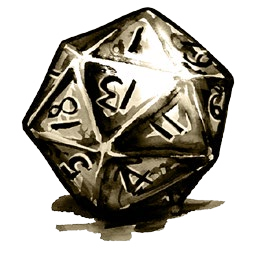
\includegraphics[width=0.5\linewidth]{würfel20.png}
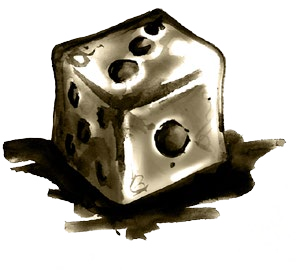
\includegraphics[width=0.3\linewidth]{würfel6.png} 
%
	Bilder werden mit \begriff{includegraphics} eingefügt. Wenn man keine Zeile frei lässt, werden sie im laufenden Text eingefügt, mit freier Zeile davor und danach stehen sind sie Blockelemente.
	Die Breite sollte in den Optionen mit \emph{[width=0.xx\textbackslash{}linewidth]}  angegeben werden. 
	 Siehe hier im Quelltext. 

	An Menschen mit \LaTeX-Erfahrung aus der Uni:
     Anders als bei wissenschaftlichen Arbeiten sollten Bilder nicht in eine \emph{figure}-Umgebung eingebettet werden;
	 dadurch erscheint das Bild auch genau da, wo ihr es definiert habt.

\subsubsection{Eine besonders lange Subsection um auch das einmal zu zeigen}
Es können in XeLaTeX beliebige UTF8-Zeichen eingefügt werden: Beispielweise: 
	\emph{Erschwernisse und Erleichterungen betragen immer ±2, ±4, ±8, ±16.}

\begin{kasten}{4.8cm}{Erklärkästen}
	Ein Kasten wird mit der Umgebung \begriff{kasten} eingefügt ;) Als Zwingende Elemente werden die Üerschrift und die Kastenhöhe erwartet – hier ist auch \emph{\textbackslash{}textheight} als Höhe möglich für die gesamte Seitenhöhe.  
	Absätze funktionieren auch in Kästen.

	\minisec{Weitere Überschriften im Kasten mit \emph{minisec}}
	\textsc{Achtung:} Vor einem Kasten sollte eine Leerzeile stehen, sonst verrutscht er nach rechts! Nach dem Kasten nicht, damit es keinen Einzug gibt.
\end{kasten}

Hier geht es dann mit weiterem Text weiter. Oder einer neuen Überschrift.

\subsection{Drucken}
Es ist möglich, den Hintergrund beim Drucken auszublenden.
Ebenso wurde mal im Forum angefragt, ob man die Kästen durch einen Rahmen ersetzen könnte für den Druck.
Dies ist in dieser Version möglich mit allen PDF-Readern, die Ebenen/Layers unterstützen (beispielsweise \emph{Acrobat Reader} und \emph{Evince})
\footnote{Falls du keinen hast hier ein \href{https://www.pdftron.com/webviewer/demo}{online Viewer} um es mal zu testen.}.
Die Ebenen heißen \emph{Hintergrund}, \emph{Kasten} und \emph{Rahmen-statt-Kasten} (deaktiviert).


\clearpage % Um eine neue Seite zu beginnen und die Spalte zu beenden.

% % ----------------------
% % Falls eine "linke" Spalte frühzeitig beendet werden muss, ohne dass sie sich bis nach unten füllt und unschöne Lücken reisst:
% \vfill  
% \	% <-- Dieses Leerzeichen braucht vfill um etwas vor dem Spaltenumbruch zum Auffüllen zu haben.
% 	%     Ohne vfill + \ wird die Spalte bis nach unten gestreckt. Am besten columnbreak nur selten benutzen.
% \columnbreak
 
\subsection{Weitere Befehle}

Es gibt zudem noch den neuen Befehl \begriff{begriff} der im Endeffekt jetzt nur Fett aktiviert. In der ersten Planung war geplant das Regelwerk mit dieser Vorlage nachzubauen. Dann hätte ebenfalls ein Index erstellt werden sollen – hauptsächlich aus den mit \begriff{begriff} markierten Wörten.

Einen Spaltenumbruch erzeugt man übrigens mit \begriff{columnbreak}. Vor einem neuen Kapitel kann man mit \begriff{vfill} und einem erzwungenem Leerzeichen die letze Spalte vorzeitig enden lassen, so dass sie nicht bis zum Ende der Seite geht. 

\LaTeX\ passt den Abstand von Umgebungen (Überschriften, Listen, Paragraphen) dynamisch an, manchmal sind daher die Abstände größer als man sie gerne hätte. Dann kann man mit bestimmten Befehlen Abstände einfügen (\begriff{vfill, vspace, smallskip, medskip, bigskip})

Man sollte aber erst am Ende(!) des Schreibvorgangs mit \begriff{vfill, smallskip, medskip, bigskip} Anpassungen vornehmen. Und auch nur wenn die Abstände wirklich seltsam sind (\LaTeX\ warnt mit \emph{Under-/Overfull box}). Manchmal ist es dabei sogar einfacher einfach den Text umzuformulieren ;)

Sollte es einmal nötig sein, kann man mit \begriff{noindent} den Absatz-Einzug für diesen Paragraph deaktivieren. Z.B. wenn man nach skips oder einem Kasten oder einer Graphik einen neuen Gedankengang beginnt.


\subsubsection{Tabellen}
Diese Tabelle (tabularx) passt ihre Breite automatisch an, ist aber zu breit für die Spalte und erzeugt dadurch \emph{Overfull box}-Warnungen.

\begin{tabularx}{\linewidth}{rXXX}
			  & \textbf{Zauberer} & \textbf{Geweihte} & \textbf{Paktierer} \\
	\hline
	Vorteil	  & Zauberer	 & Geweiht	   & Paktierer \\   
	Energie	  & Astralpunkte & Karmapunkte & Gunstpunkte \\ 
	Tradition & magisch	     & karmal	   & dämonisch \\   
übern.Talente & Zauber	     & Liturgien   & Anrufungen \\  
\end{tabularx}

\bigskip

Diese Tabelle ist eine normale \LaTeX\ \emph{tabular}. Sie erfordert mehr Handarbeit, dafür kann sie feinstufiger angepasst werden.


% Normale Tabelle ohne tabularx
\begin{tabular}{l@{ }c@{\ }c@{\ }c}
			  & \textbf{Zauberer} & \textbf{Geweihte} & \textbf{Paktierer} \\
	\hline
	Vorteil	  & Zauberer	 & Geweiht	   & Paktierer \\
	Energie	  & Astralpunkte & Karmapunkte & Gunstpunkte \\
	Tradition & magisch	     & karmal	   & dämonisch \\
übern.Talente & Zauber	     & Liturgien   & Anrufungen \\
\end{tabular}
\end{multicols}

\vfill

\section*{Großes Tabellenbeispiel}
Außerhalb der multicols-Umgebung über die gesamte Seite.%
\footnote{Die große Tabelle ist mit zwei \begriff{vfill} „mittig“ zentriert worden.}

\bigskip

\begin{tabularx}{0.98\linewidth}{p{3cm}XX}
	\textbf{Vorraus.} & \textbf{Eigenschaft1} & \textbf{Eigenschaft2} \\
	\hline
	Attribut 4 \newline 20 EP  & \minisec{Extra Cool} Eine Sonderfähigkeit                  & \minisec{Extra Cool} Eine Sonderfähigkeit \\
	Attribut 6 \newline 40 EP  & \minisec{Aufbauend} Ein weiterer Bonus mit ganz viel Text
								 um das Verhalten der restlichen Tabelle darauf zu sehen.
								 Blabablablablabla                                          & \minisec{Tabellenzauberer} Perfekte Tabellen \\
	Attribut 8 \newline 120 EP & \minisec{Final} \emph{Godmode activate}                    & Hier mal was ohne Überschrift \\
	\hline
\end{tabularx}

\vfill

\cleardoublepage


\addchap{Planungen}
	\noindent Das folgende werde ich noch in einer Version zwei nachreichen, wenn dies gewünscht ist - oder ich nicht lang genug stillhalten kann: 
	\begin{itemize}
		\item Eine Möglichkeit den Hintergrund auszublenden, wie im Originaldokument (Lösungsansatz dafür ist schon bekannt) \vfill \textsc{[Erledigt]}
		\item Passendes Schriftdesign im Inhaltsverzeichnis, \vfill \textsc{[Erledigt]} (Schickt erstmal so und muss ja nicht in ner Spielhilfe unter 50 Seiten perfekt übereinstimmen)
		\item Mal Verlinkungen auf Herz und Nieren prüfen,
		\item eine Vorlage oder evtl. Umgebung für die Gegnertabellen umsetzen (Sieht irgendwie nach einer mehr oder weniger komplexen Tabelle mit Spaltenzahl 1 aus), 
		\item einen Index bzw. Glossar, der aus den \emph{Begriff}en automatisch erstellt wird.
	\end{itemize}


\begin{multicols}{2}
\vfill % Das Kasten-Bild muss sich an etwas festhalten! (Nur nötig bei Seiten-/Spaltenanfang)
\begin{kasten}{0.1\textheight}{Nachfolgend ein Kasten-Test}
	Textkasten mit 0.1 textheight \vspace{1.2cm}
\end{kasten}

\begin{kasten}{0.2\textheight}{Nachfolgend ein Kasten-Test}
	Textkasten mit 0.2 textheight \vspace{3.7cm}
\end{kasten}

\begin{kasten}{0.33\textheight}{Nachfolgend ein Kasten-Test}
	Textkasten mit 0.33 textheight 
\end{kasten}

\vfill
\ 
\columnbreak

\begin{kasten}{0.65\textheight}{Was stellen Erfahrungspunkte dar?}
EP sind ein grobes Maß für die Fähigkeiten deines 
Charakters und eine Belohnung für dich, mit der du 
deinen Charakter verbessern kannst. 

Sie können und sollen nicht das reale Lernen eines 
Aventuriers simulieren. Deswegen gibt es keine EP für 
monatelanges Studieren in Bibliotheken und die Kosten 
aller Fähigkeiten messen sich nur an deren Nutzen, nicht 
daran, wie schwierig sie zu erlernen sind. 

\minisec{Erfahrungspunkte für Nichtspielercharaktere?}
Nichtspielercharaktere (NSC) folgen in Ilaris denselben 
Charakterregeln wie Spielercharaktere, müssen also zum 
Beispiel die Voraussetzungen von Vorteilen erfüllen. 
Trotzdem wird es in den meisten Fällen genügen, 
die Werte von NSC entsprechend ihrer geplanten 
Vorteile werden „auf einen Schlag“ erworben. Entweder
dein Charakter besitzt einen Vorteil – oder eben nicht. Je
nach Macht und Vielseitigkeit kosten sie 20, 40, 60, 80 oder
100 Erfahrungspunkte und besitzen manchmal spezielle
Voraussetzungen.
\begin{itemize}
	\item  Du benötigst einen Vorteil, der deinem Charakter
		seine übernatürliche Energie zur Verfügung stellt.
		Beispielsweise müssen Zauberer den Vorteil Zauberer
		kaufen, der ihnen Astralpunkte (AsP) verleiht.
	\item  Zusätzlich musst du einen Traditionsvorteil erwerben,
		mit der du deine übernatürlichen Fähigkeiten einsetzen
		kannst. Beispielsweise würde ein Zauberer eine magische
		Tradition, wie die der Druiden, erwerben.
	\item  Zuletzt steigerst du noch übernatürliche Fertigkeiten und
		Talente. Letztere sind einfach ein Sammelbegriff für Zauber, Liturgien und Anrufungen. Beispielsweise könnte ein Druide die übernatürliche Fertigkeit „Einfluss“ steigern,
		und dafür die übernatürlichen Talente (bzw. Zauber) Böser
		Blick und Herr über das Tierreich freischalten.
\end{itemize}
\end{kasten}
\end{multicols}

